% Tikz File 'model640.tex'
\documentclass{standalone}

\usepackage{tikz} %Graphics
\usetikzlibrary{shapes.geometric, arrows}
\tikzstyle{title} = [text centered]
\tikzstyle{block} = [rectangle, rounded corners, minimum width=3cm, minimum height=1cm,text centered, draw=black, fill=blue!30]
\tikzstyle{conv} = [rectangle, rounded corners, minimum width=3cm, minimum height=1cm,text centered, draw=black, fill=blue!30]
\tikzstyle{batchnorm} = [rectangle, rounded corners, minimum width=3cm, minimum height=1cm,text centered, draw=black, fill=green!30]
\tikzstyle{relu} = [rectangle, rounded corners, minimum width=3cm, minimum height=1cm,text centered, draw=black, fill=orange!30]
\tikzstyle{maxpool} = [rectangle, rounded corners, minimum width=3cm, minimum height=1cm,text centered, draw=black, fill=red!30]
\tikzstyle{arrow} = [thick,->,>=stealth]

%\usetikzlibrary{...}
\begin{document}
		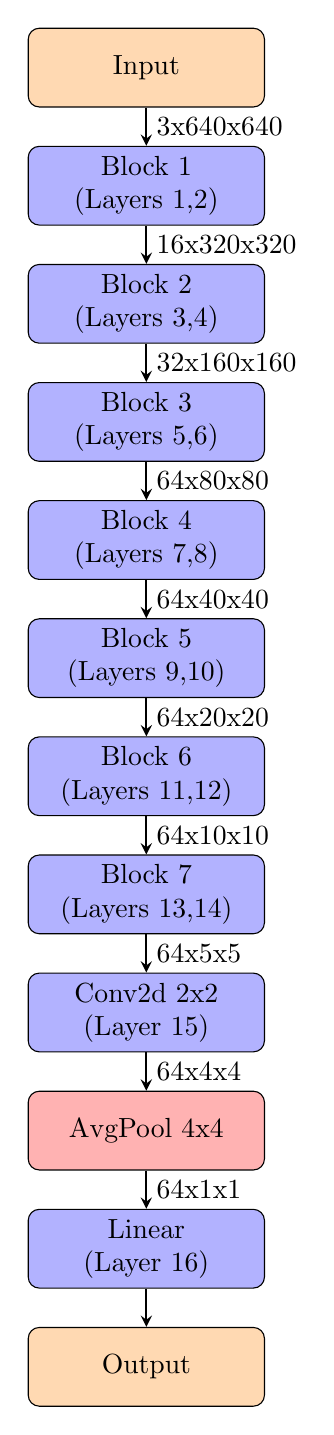
\begin{tikzpicture}[node distance=1.5cm]
				\node (i1) [relu] {Input};							% 640x640
				\node (b1) [block, below of=i1, align=center] {Block 1 \\ (Layers 1,2)};
				\node (b2) [block, below of=b1, align=center] {Block 2 \\ (Layers 3,4)};
				\node (b3) [block, below of=b2, align=center] {Block 3 \\ (Layers 5,6)};
				\node (b4) [block, below of=b3, align=center] {Block 4 \\ (Layers 7,8)};
				\node (b5) [block, below of=b4, align=center] {Block 5 \\ (Layers 9,10)};
				\node (b6) [block, below of=b5, align=center] {Block 6 \\ (Layers 11,12)};
				\node (b7) [block, below of=b6, align=center] {Block 7 \\ (Layers 13,14)};
				\node (b8) [conv, below of = b7, align=center] {Conv2d 2x2 \\ (Layer 15)};
				\node (av15) [maxpool, below of=b8] {AvgPool 4x4};	% 1x1
				\node (linear) [conv, below of=av15, align=center] {Linear \\ (Layer 16)};	% 1x1
				\node (output) [relu, below of=linear] {Output};	
				
				\draw [arrow] (i1) -- node [right, midway] {3x640x640} (b1);
				\draw [arrow] (b1) -- node [right, midway] {16x320x320} (b2);
				\draw [arrow] (b2) -- node [right, midway] {32x160x160} (b3);
				\draw [arrow] (b3) -- node [right, midway] {64x80x80} (b4);
				\draw [arrow] (b4) -- node [right, midway] {64x40x40} (b5);
				\draw [arrow] (b5) -- node [right, midway] {64x20x20}  (b6);
				\draw [arrow] (b6) -- node [right, midway] {64x10x10}  (b7);
				\draw [arrow] (b7) --  node [right, midway] {64x5x5}  (b8);
				\draw [arrow] (b8) --  node [right, midway] {64x4x4} (av15);
				\draw [arrow] (av15) --  node [right, midway] {64x1x1} (linear);
				\draw [arrow] (linear) -- (output);		
		\end{tikzpicture}
\end{document}
